\documentclass{beamer}
\usepackage{beamerthemesplit}
\usepackage{graphics}
\usepackage{pstricks}
\usepackage[T2A]{fontenc}			% кодировка
\usepackage[utf8]{inputenc}			% кодировка исходного текста
\usepackage[english,russian]{babel}	% локализация и переносы
%grek
\usepackage{ tipa }
\usepackage{ amssymb }

\usepackage{caption, subcaption}
\usepackage{wasysym}
%\usepackage{enumitem}
\graphicspath{ {img/} }


\title{Кафедра нанометрологии и наноматериалов}
\author{Михаил Соловьянов}


\begin{document}


\frame{
   \begin{center}
    \huge{Создание энергоэффективных блоков сегнетоэлектрической памяти для нейроморфных приложений}\\
    \vspace{24pt}
    \Large{Научный руководитель: Дмитрий Владимирович Негров}\\
    \vspace{14pt}
    \Large{Соловьянов Михаил Михайлович}\\
    \vspace{24pt}
    \large{\today}
  \end{center}
}






\frame{\frametitle{Постановка задачи}
 \begin{center}
  \begin{enumerate}
   \item Разработать тестовый прототип FRAM памяти на новом сверхтонком слое сегнетоэлектрика, включающий в себя так же цифровой контроллер памяти.
   
   \item Подготовить layout на базе существующей технологии для создания устройства. 
  \end{enumerate} %на самом деле задач было больше, но они не уместились на слайд!
 \end{center}
}





\frame{
 \begin{center}
\bf{Почему FRAM в лаборатории нейровычислительных систем?}
 \end{center}
}


\frame{\frametitle{Сегнетоэлектрик из HfO2-ZnO2}
 \begin{center} 
 \begin{figure}
 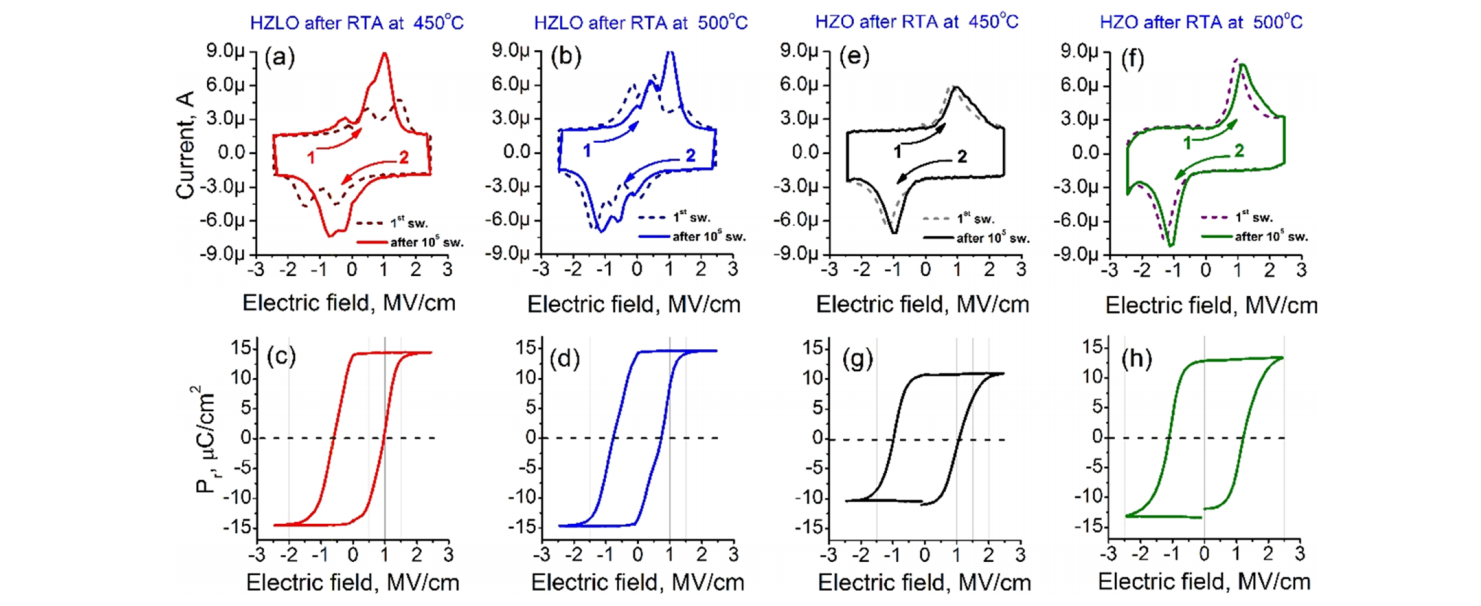
\includegraphics[width=0.90\textwidth]{graph0.png}
 \caption{Графики Поляризации от внешнего поля и ток через элемент при переполяризации, полученные в лабораториях ЦКП в 2016 году }
 \end{figure}

 \end{center}
}

%$Hf_{0.5}Zr_{0.5}O_2$

\frame{\frametitle{Строение Ferroelectric Random Access Memory (FRAM) }
 \begin{center}

 
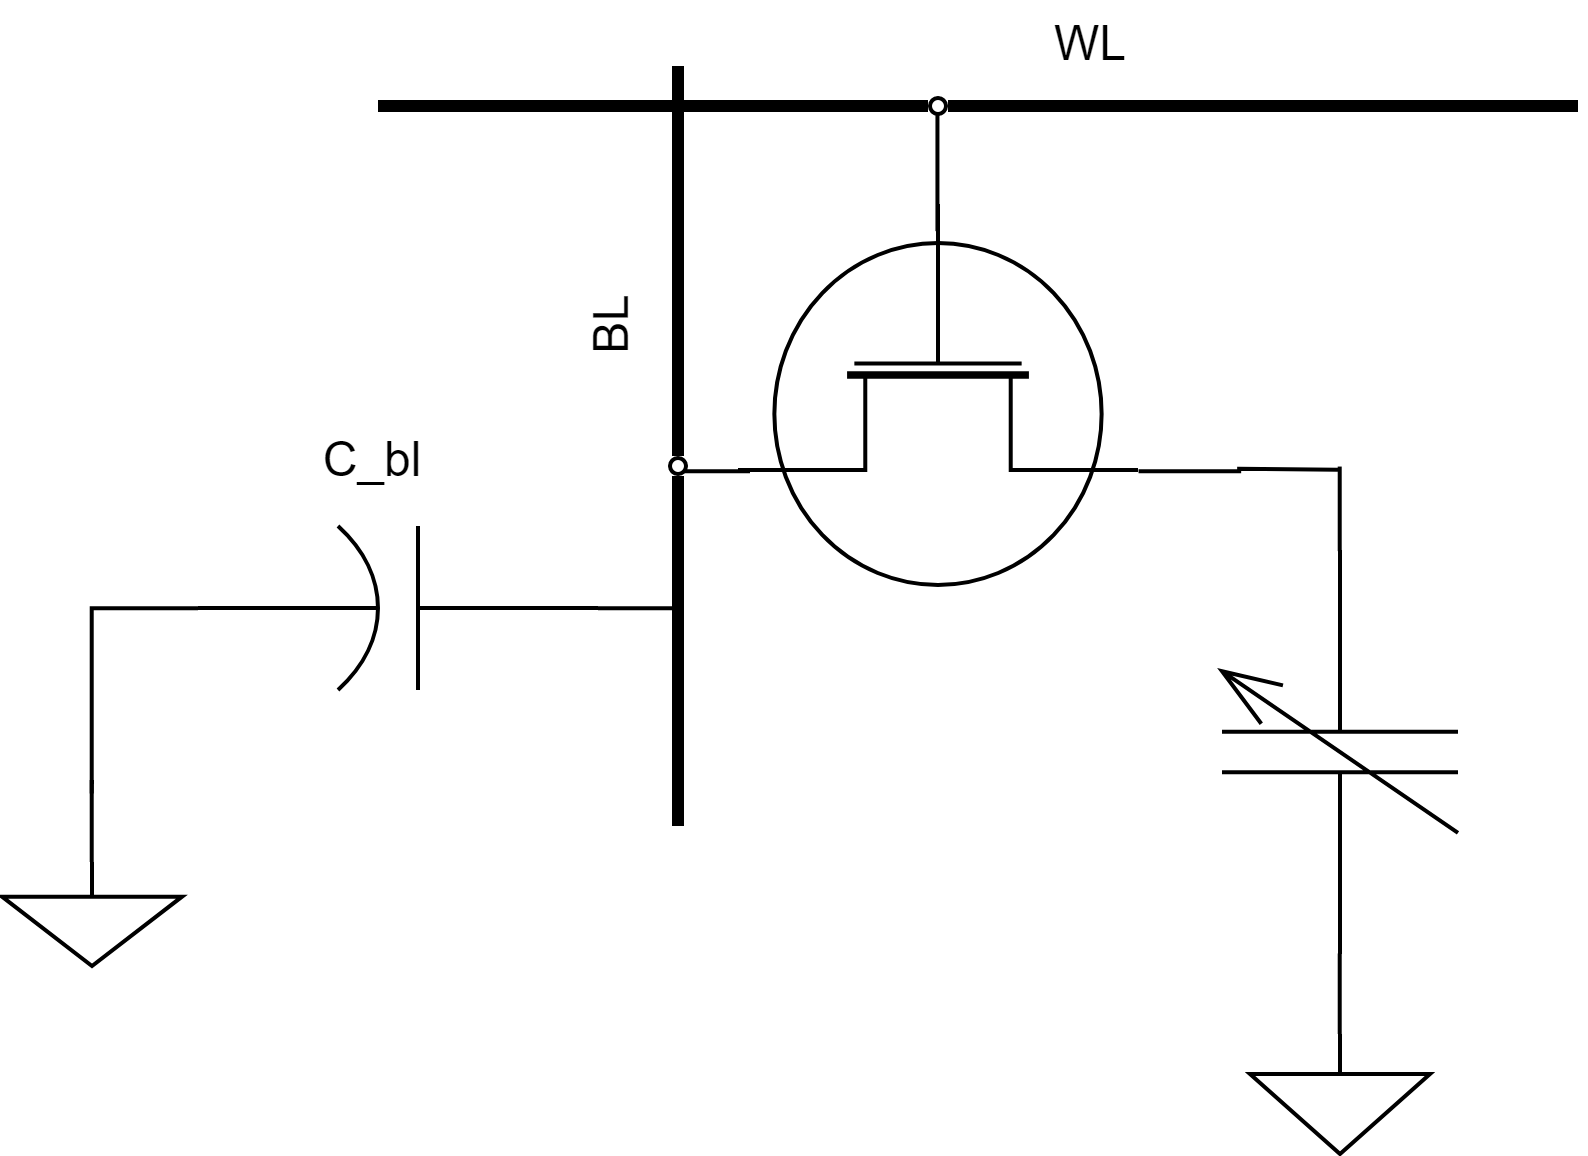
\includegraphics[width=0.95\textwidth]{FRAM-FRAM.png}

 \end{center}
}











\frame{\frametitle{Симуляция поведения cегнетоэлектрика}
 \begin{center}
 
 {\bf Что есть сегнетоэлектрик?  }  
 
 
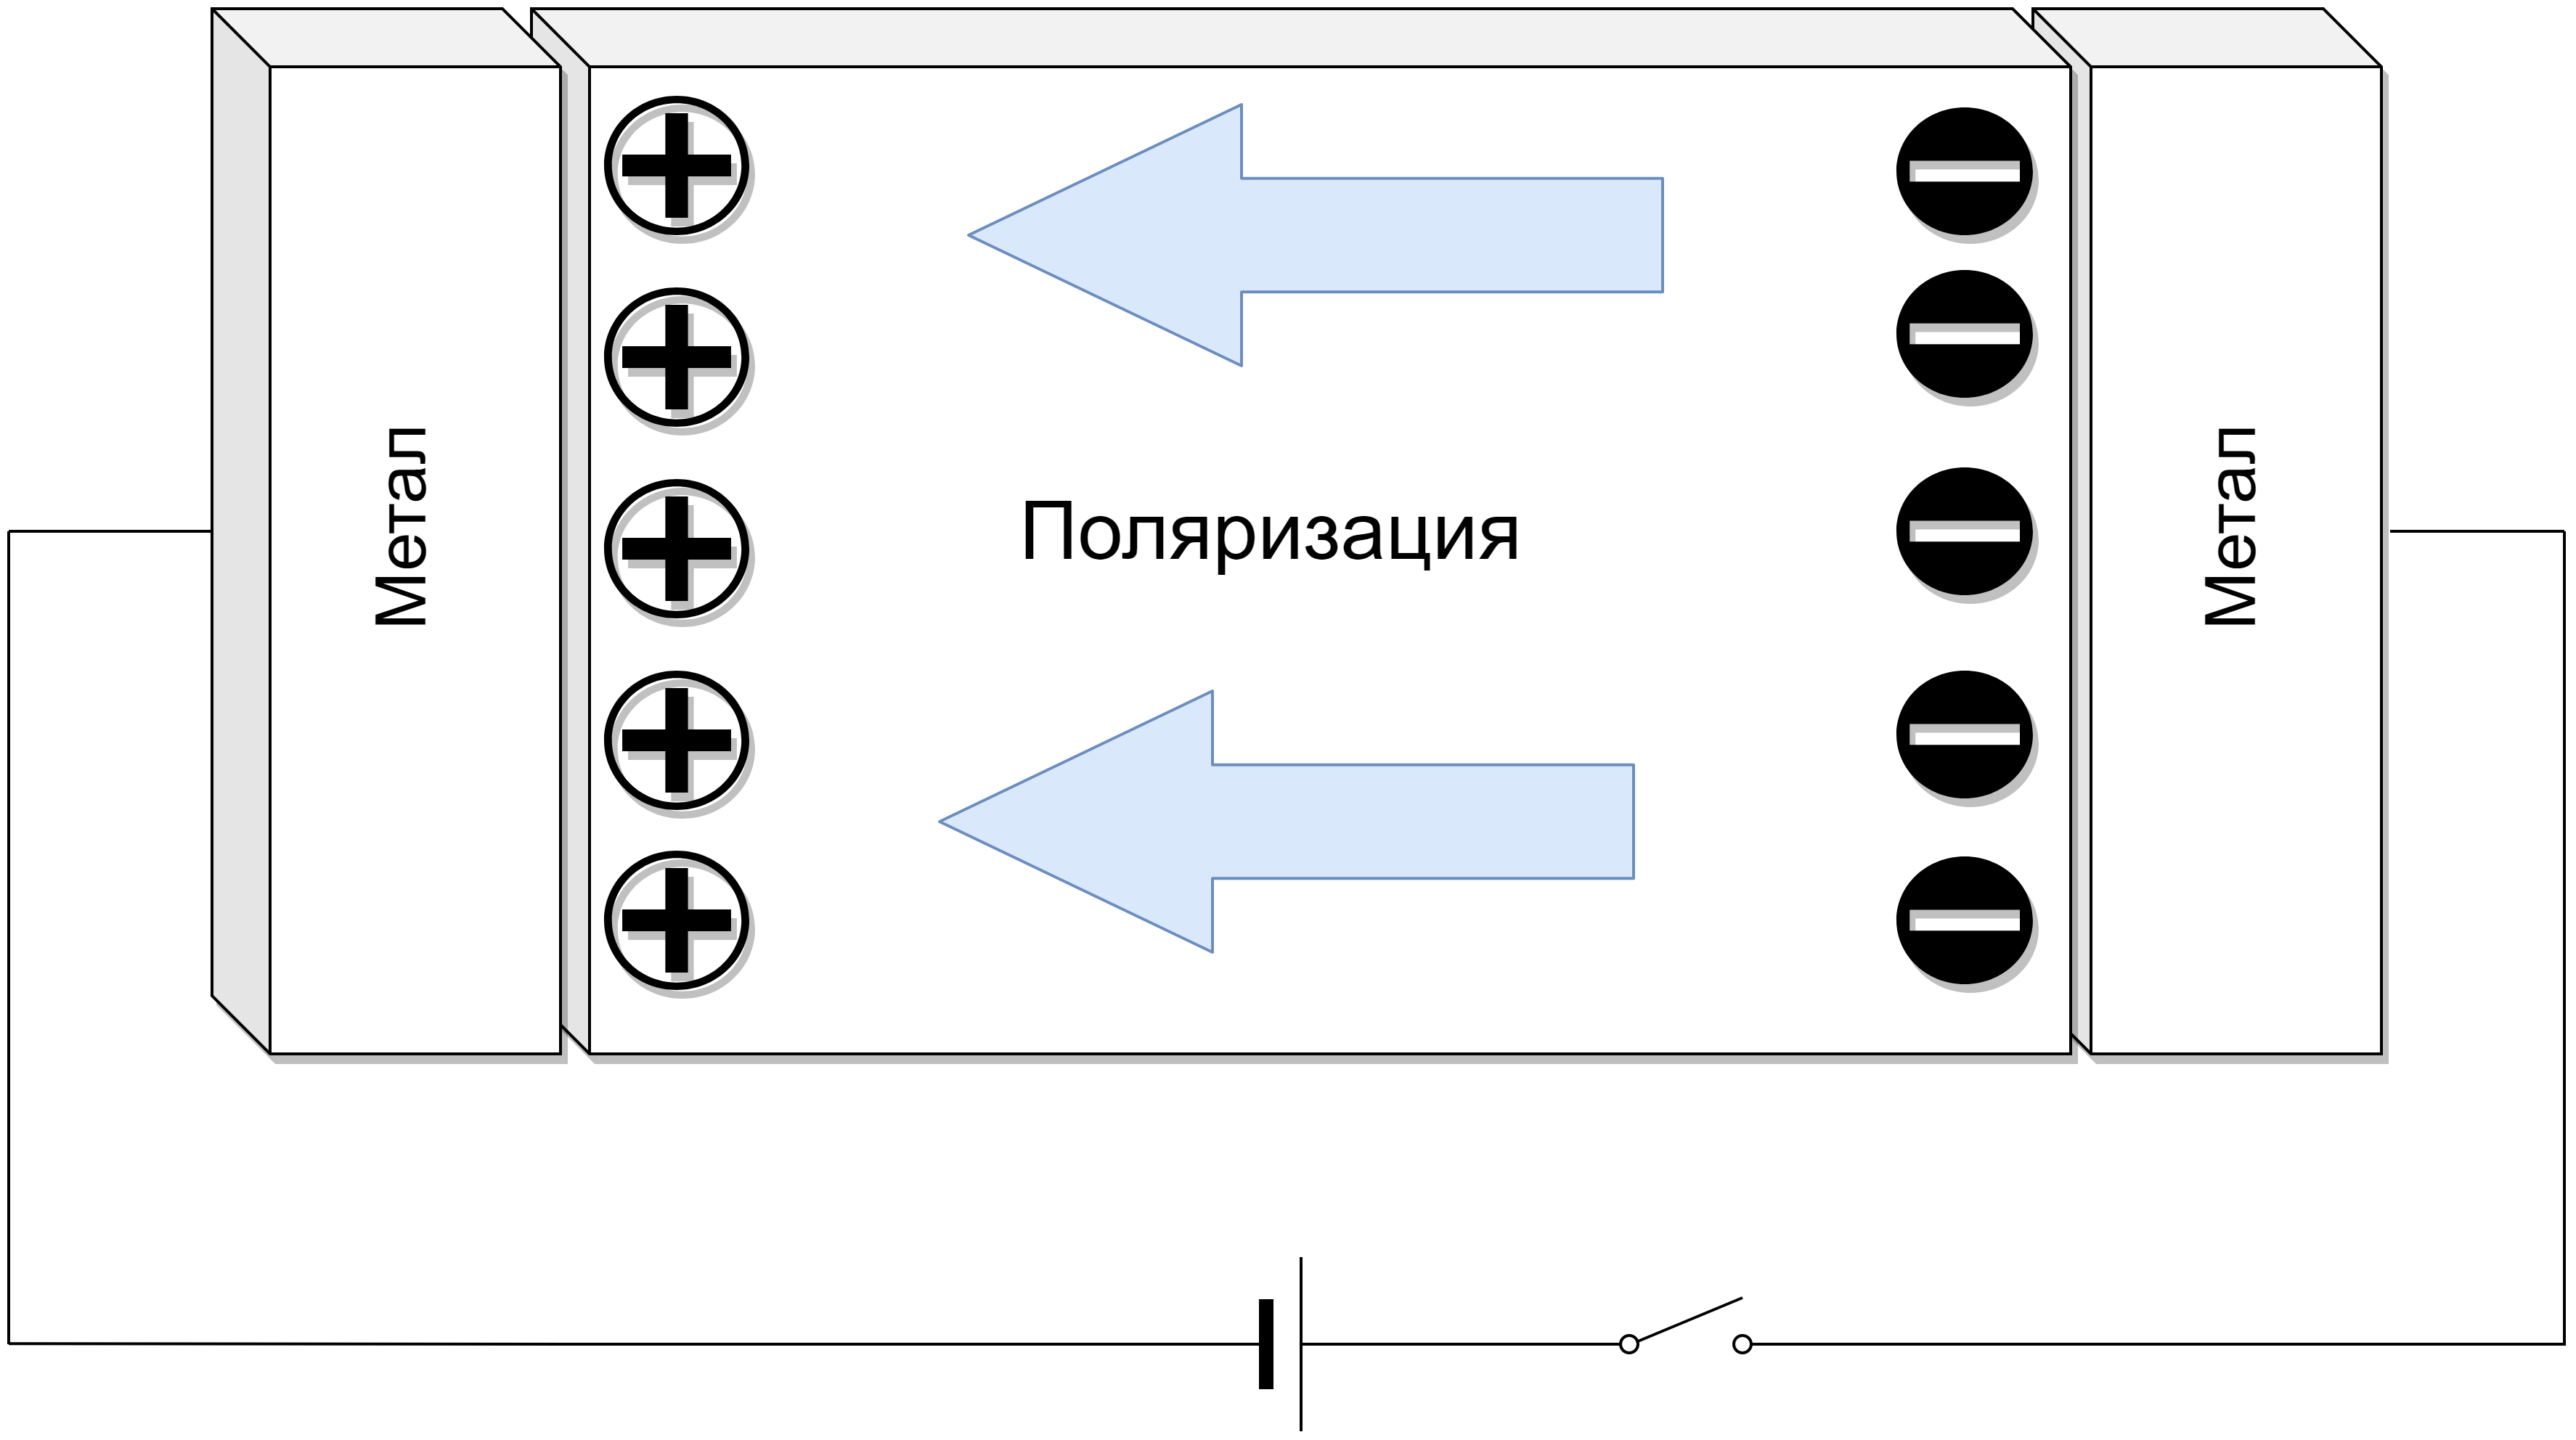
\includegraphics[width=0.90\textwidth]{FRAM-Page-4.png}
 \end{center}
}

\frame{\frametitle{Что есть сегнетоэлектрик?}
 \begin{center}
  {\bf  В физике сегнетоэлектрик -- это материал обладающий перманентной поляризацией, причем таких состояний у него два, и он способен переходить из одного в другое под действием поля. Где поляризацию можно считать Дипольным моментом системы. }\\
  
  $ \vec{P} = \sum_{j}Q_j\vec{R_j}   $
 \end{center}
}








\frame{\frametitle{Построение модели сегнетоэлектрика. Теория Ландау О фазовых переходах. }
 \begin{center}

  \begin{equation}\label{fermi}
   \mathcal{F} = \frac{1}{2}\alpha \vec{P}^2 + \frac{1}{4}\beta \vec{P}^4 - \vec{E}\vec{P}
  \end{equation}
 Где $ -EP  $ есть энергия внешнего электрического поля: с напряженностью E, находим ее из напряжения, зная толщину сегнетоэлектрика $U= \vec{E}d $.

 \end{center}
}





\frame{  
  \begin{center}
  	График зависимости $\mathcal{F}(P) $  и его связь с гистерезисом. Сама энергия без внешнего поля стремится в локальный минимум (ноль производной).
    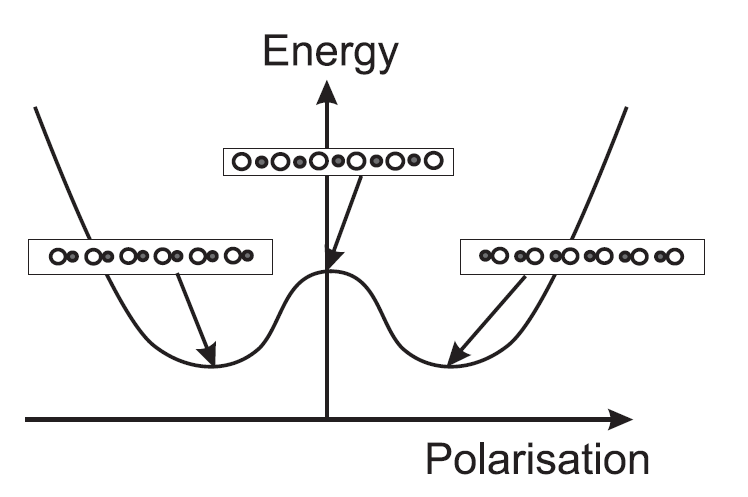
\includegraphics[width=0.5\textwidth]{F(P).png}%
	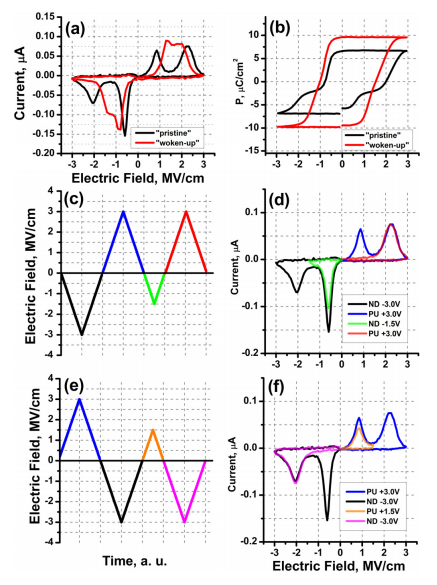
\includegraphics[width=0.5\textwidth]{Hyst.png}
  \end{center}
}

\frame{
 \begin{center}
  Дифференцируя выражение \eqref{fermi} получаем:
  \begin{equation}\label{dfermi}
  \frac{\partial \mathcal{F}}{\partial P }  = \alpha P + \beta P^3 - E
  \end{equation}
  
  
  \begin{figure}
  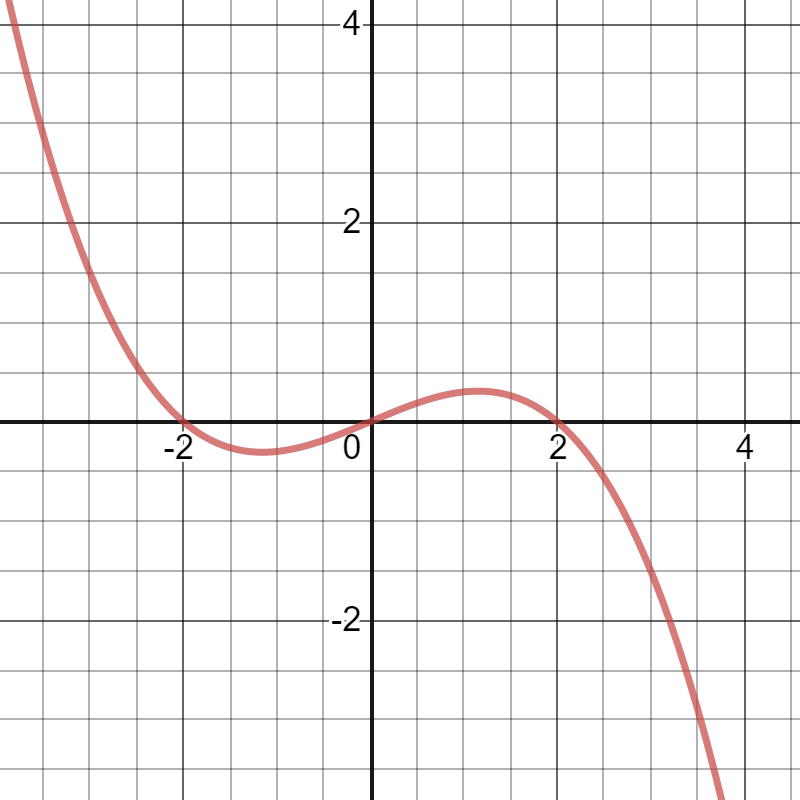
\includegraphics[width=0.55\textwidth]{graph1.png}
  \caption{Примерный график первой производной энергии}
  \end{figure}
  
 \end{center}
}


\frame{
  \begin{center}
  Для того, чтобы построить гистерезис, нужно найти связь свободной энергии $\mathcal{F} $ с производной поляризации по времени ( чтобы интегрировать/дифференцировать ее).
	 \begin{equation}\label{Rfermi}
		 \frac{\partial  \mathcal{F} }{\partial P} = - R  \frac{\partial  P }{\partial t}  
 	 \end{equation}    
 	 Где $ R $ -- аналог сопротивления, есть что-то вроде временной константы, и  выбирается исходя из экспериментально ожидаемого характерного  времени реакции системы.
  \end{center}
}



\frame{
 \begin{center}
		Осталось связать заданные нами переменные $\alpha $ и   $\beta $ с физичными, измеримыми величинами: $ \vec{E}_c $ и
		  $\vec{P}_0 $ :
		разрешая уравнение второй производной для минимума энергии ( $ \frac{\partial\mathcal{F} }{\partial \vec{P}} $ ) , и пользуясь соотношением (2) для поиска коэрцитивного напряжения, получаем:\\
		$$\alpha = 3\sqrt{3E_c/(8{P_0}^3)}$$\\
	$$ \beta = -3\sqrt{3E_c/(4P_0)}$$\\
 \end{center}
}








\frame{
 \begin{center}
  Приравнивая выражение  \eqref{dfermi} к \eqref{Rfermi} получаем :
  
  \begin{equation}
  -R \dot{\vec{P}}  = \alpha \vec{P} + \beta \vec{P}^3 - \vec{E}
  \end{equation}
  Теперь, решая это уравнение относительно заданного нами  $ t $, строим график в виде $P (E(t))$:
  \begin{figure}
  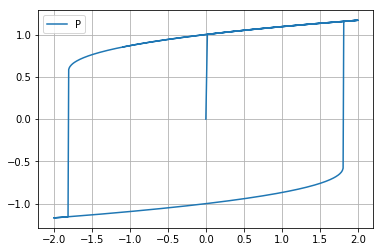
\includegraphics[width=0.7\textwidth]{Python-sym.png}
  \caption{Результат построения графика поточечного дифференцирования в Python для $ U = 2*sin(t) $}
  \end{figure}
 \end{center}
}









\frame{\frametitle{Конструкция усилителя чтения }
       \begin{tabular}{cl}  
         \begin{tabular}{c}
           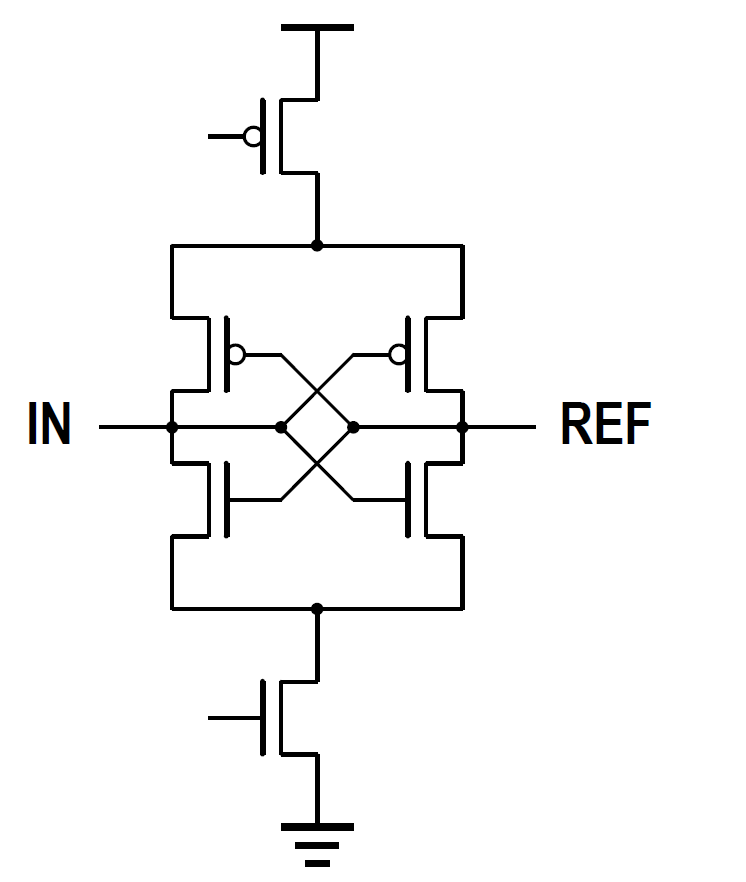
\includegraphics[height=5cm, width=3.5cm]{latch.png}
           \end{tabular}
           & \begin{tabular}{l}
             \parbox{0.5\linewidth}{%  change the parbox width as appropiate
         \bf{Популярная конструкция усилителя чтения состоит из 6T инверторной защелки, по принципу напоминающей SRAM}
    }
         \end{tabular}  \\
\end{tabular}
}




\frame{\frametitle{Конструкция усовершенствованного дифференциального неразрушающего  усилителя чтения }
 \begin{center} 

       \begin{tabular}{cl}  
         \begin{tabular}{c}
            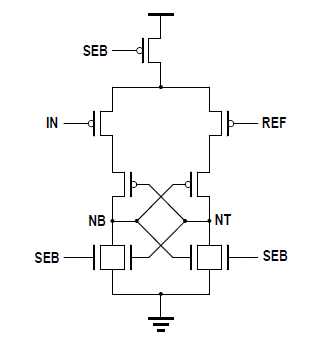
\includegraphics[width=0.5\textwidth]{SA.png}
           \end{tabular}
           & \begin{tabular}{l}
             \parbox{0.4\linewidth}{%  change the parbox width as appropiate
         Преимущество данного усилителя, в неразрушающем чтении, что дает возможность интегрировать на чип аналого-цифровой преобразователь, генерируя набор входных напряжений для сравнения.
    }
         \end{tabular}  \\
\end{tabular}
 \end{center}
}



\frame{
\begin{center} 
\begin{figure}
 \centering
 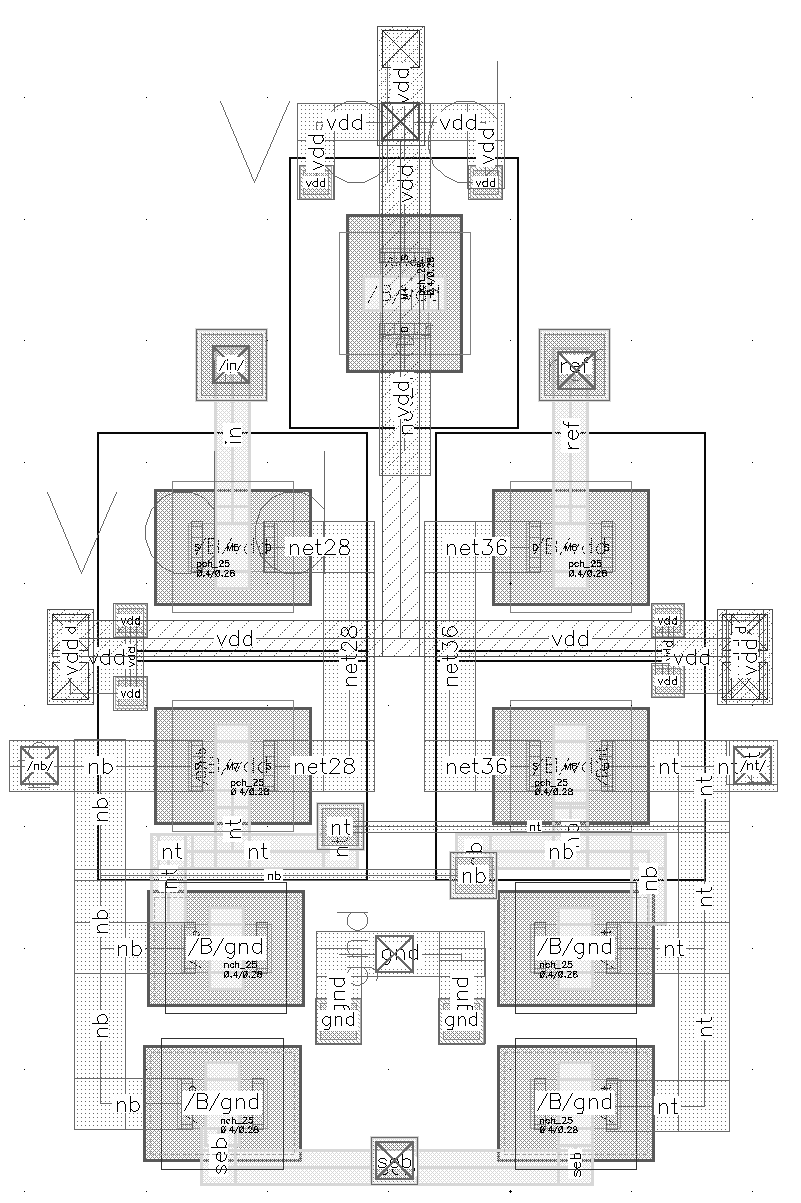
\includegraphics[width=0.9\textwidth]{AMP.png}
 \caption{ Топология дифференциального неразрушающего  усилителя чтения. }
 \end{figure}
 \end{center}
}




\frame{
 \begin{center} 
  \begin{figure}
 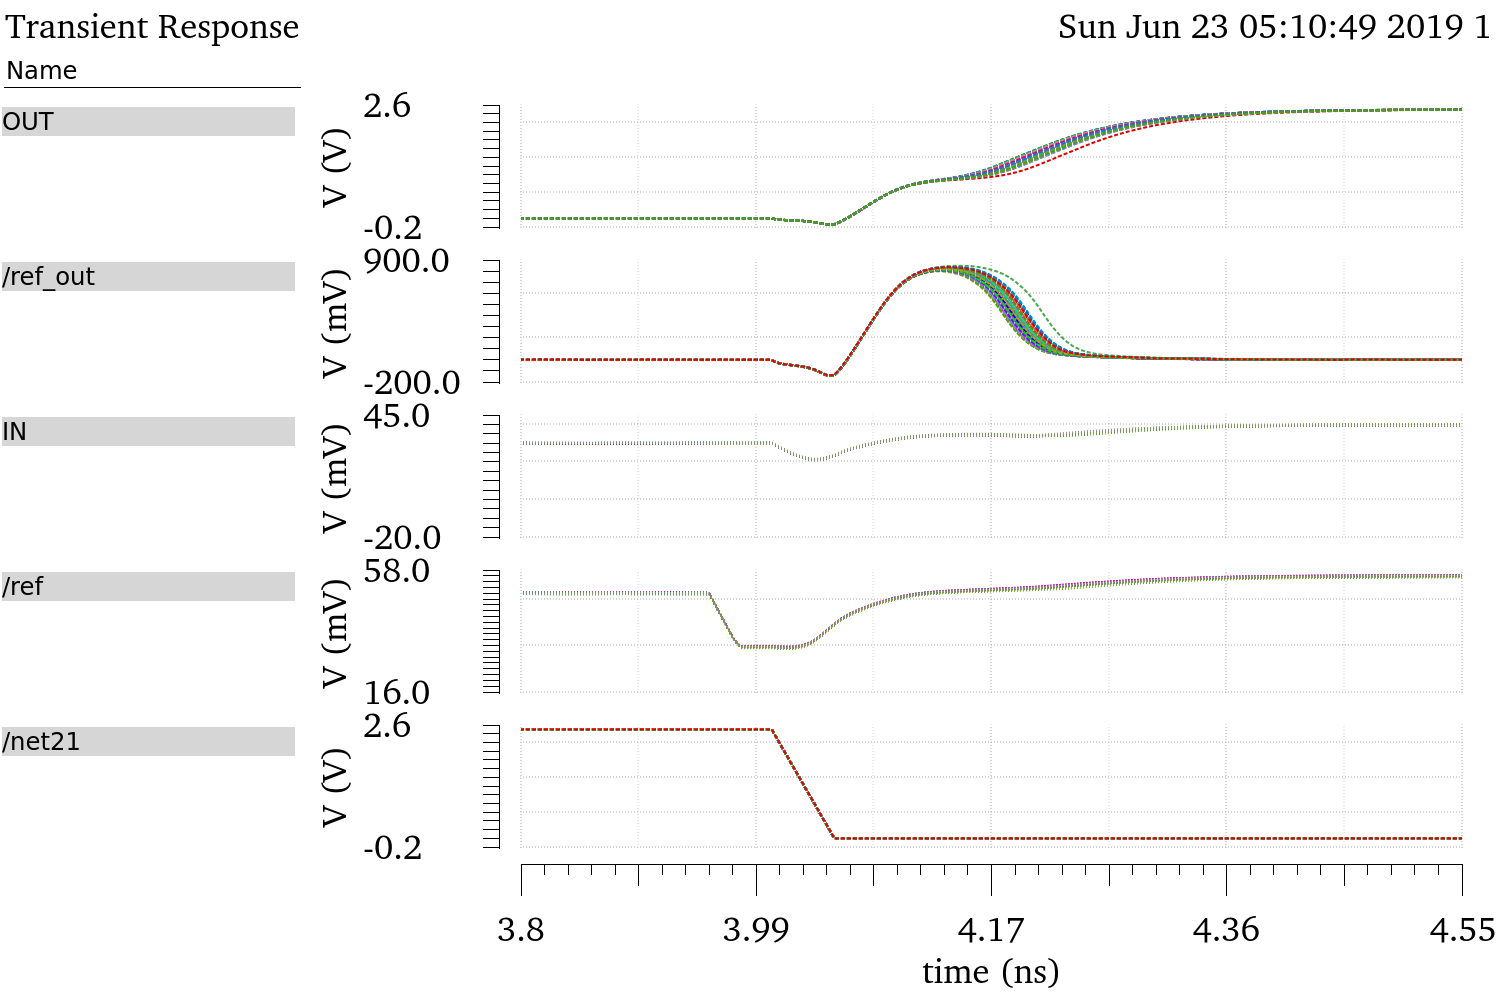
\includegraphics[width=1\textwidth]{ok.png}
 \caption{ Пример успешного сравнения зарядов. Ансамбль из 200 испытаний с учетом полосы шумов по методу Монте Карло в  САПР Cadence Virtuoso . }
 \end{figure}
 \end{center}
}

\frame{
 \begin{center} 
  \begin{figure}
 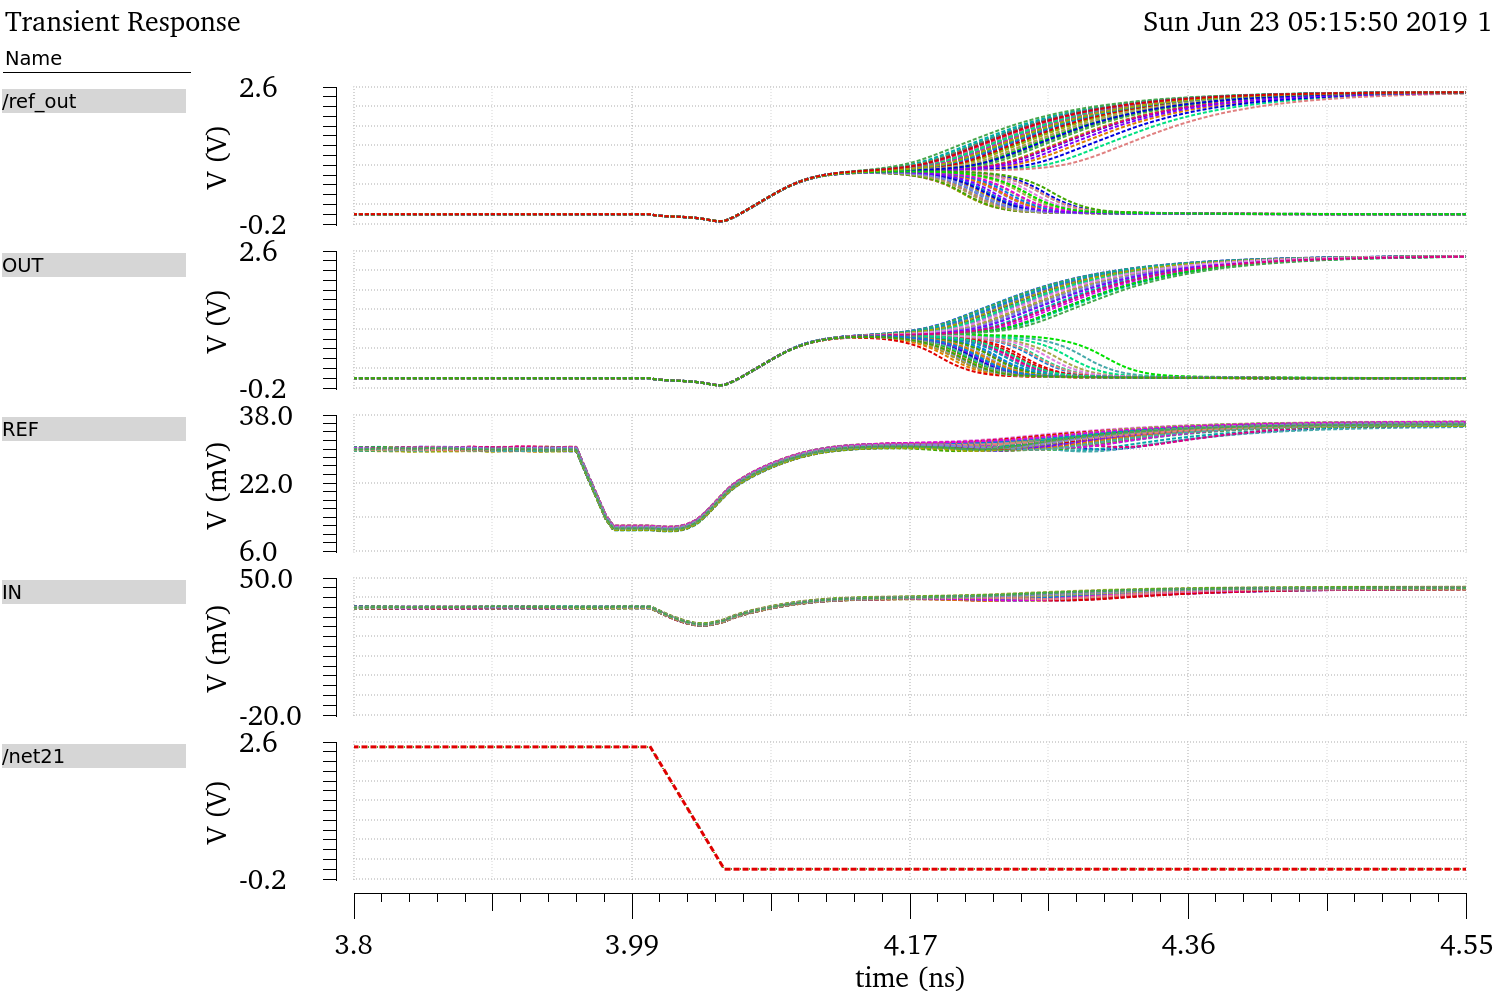
\includegraphics[width=1\textwidth]{fail.png}
 \caption{ Пример невозможности  сравнения из за влияния теплового шума.  Ансамбль из 200 испытаний с учетом полосы шумов по методу Монте Карло в  САПР Cadence Virtuoso. }
 \end{figure}
 \end{center}
}


\frame{
 \begin{center} 
 \begin{figure}
 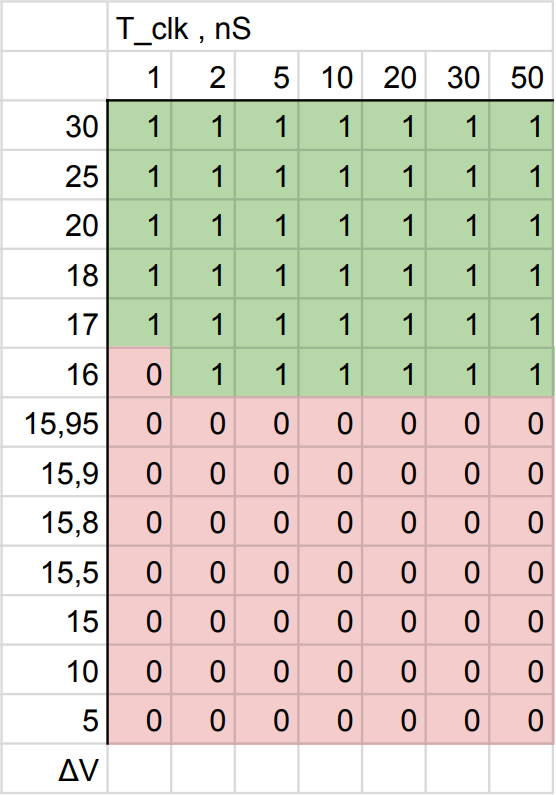
\includegraphics[width=0.45\textwidth]{shmoo.png}
 \caption{Пределы разности сравнения при $V_{ref} = 30mV $ , как видно точность измерения порядка 16 mV, определяется тепловым шумом, на различных частотах ( временная симуляция с учетом полосы шумов по методу Монте Карло в  Cadence Virtuoso)}
 \end{figure}
 \end{center}
}



\frame{\frametitle{Топология ячейки памяти}
\begin{figure}
 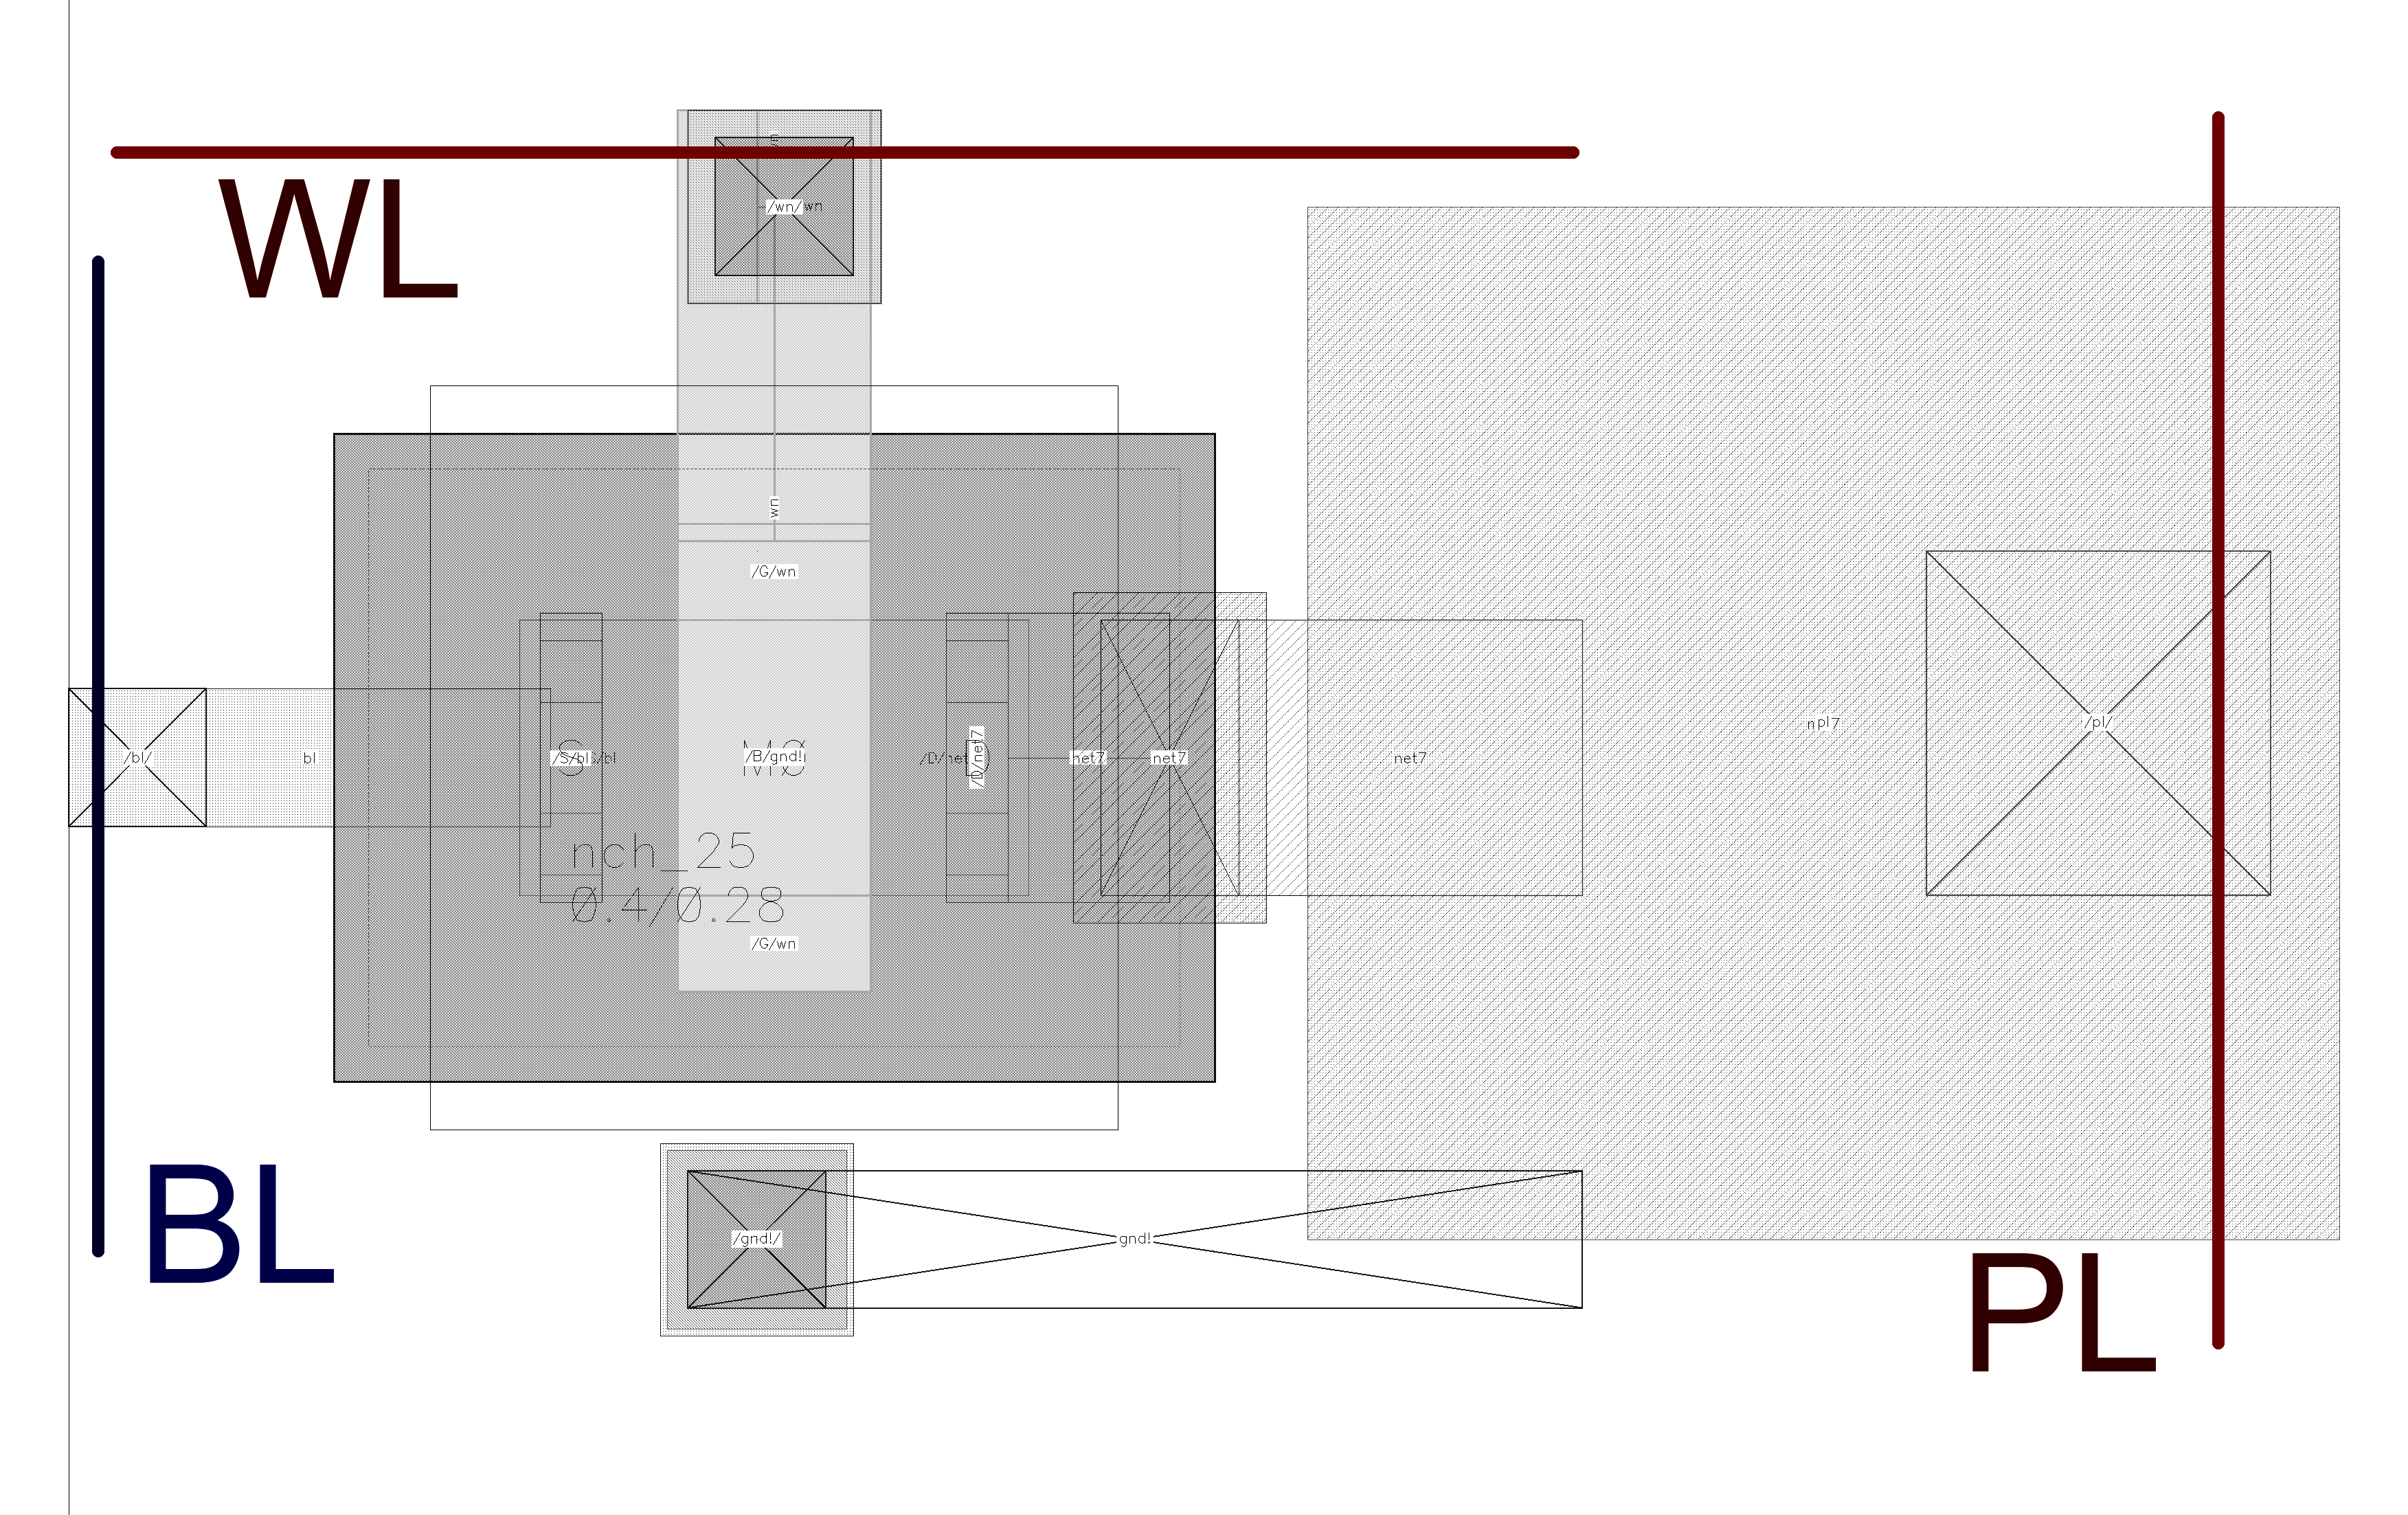
\includegraphics[width=0.9\textwidth]{cell.png}
 \caption{ Топология ячейки памяти }
 \end{figure}
}


\frame{\frametitle{ Баланс между ёмкостью линии и ёмкостью ячейки }
$$ C_{BL} \geqslant \frac{2Q_r + 2V_c C_s }{V_{PL} - V_c  } $$ 
$$ \frac{Q_r}{\Delta V_{min}} - C_s \geqslant C_{BL} $$, Формула необходимой ёмкости битлайна.

}

\frame{

\begin{figure}
 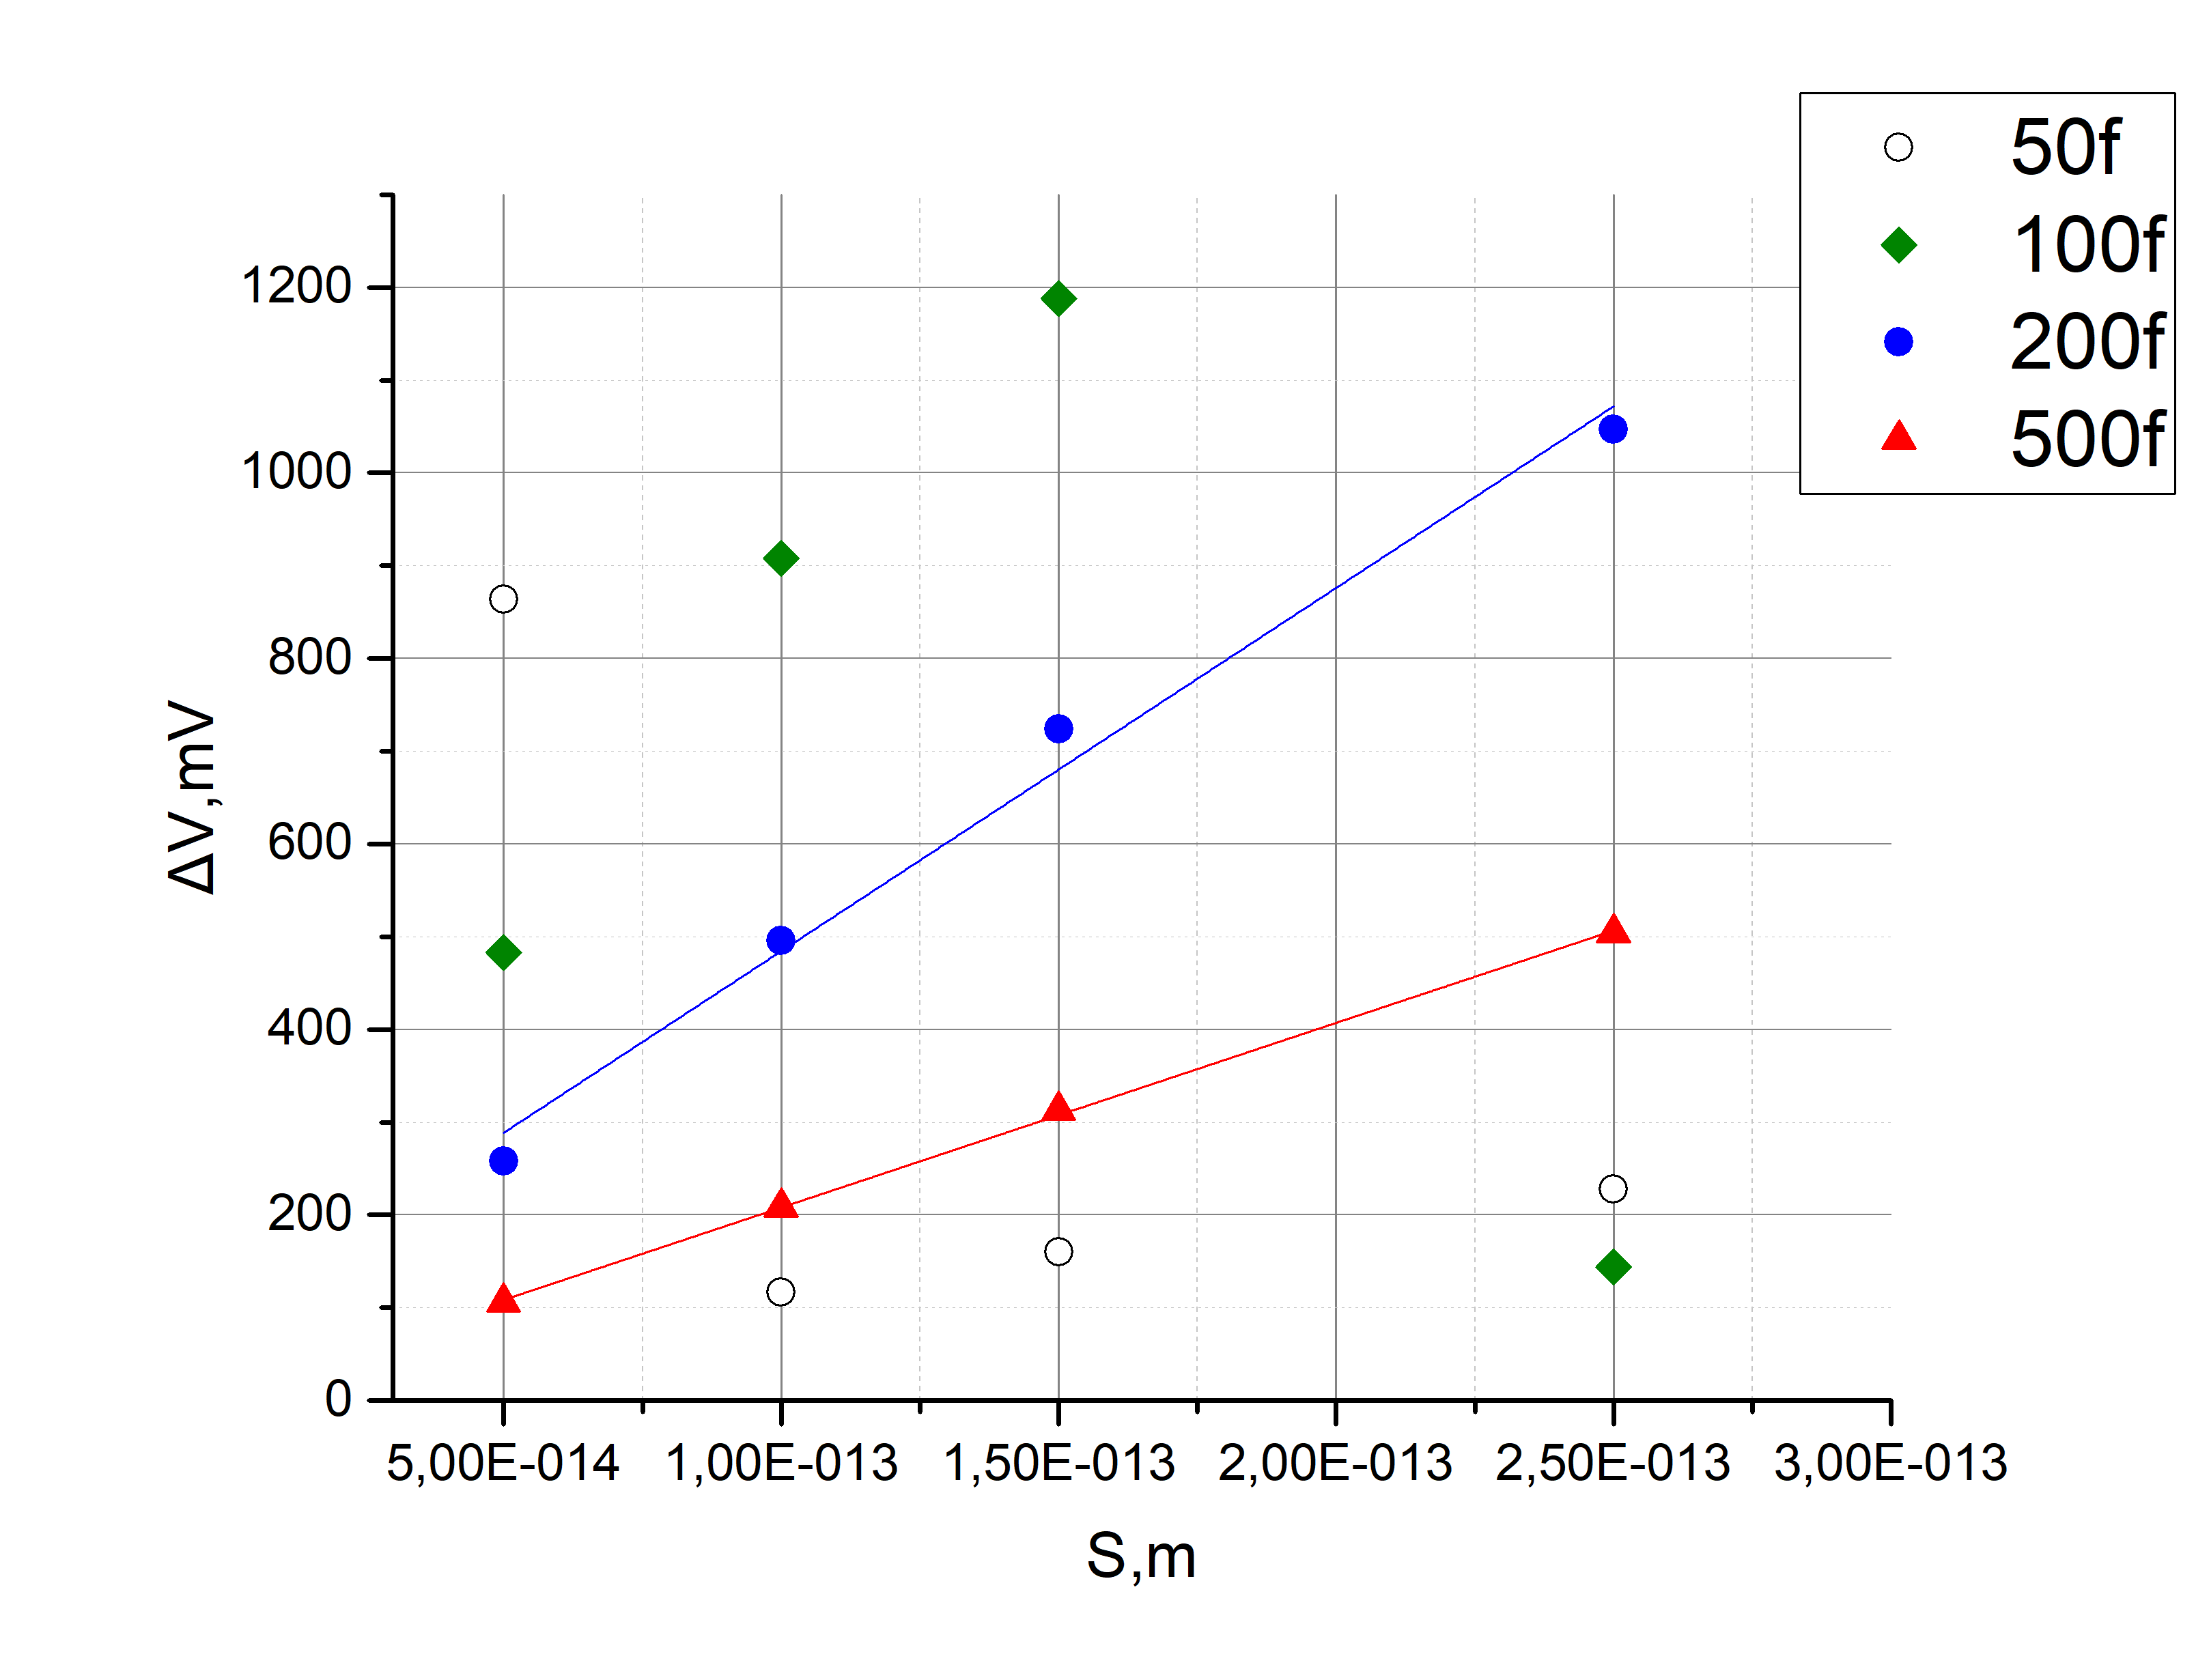
\includegraphics[width=0.7\textwidth]{c_bl.png}
 \caption{График Считываемой разности напряжений от площади ячейки. }
 \end{figure}
}




\frame{
 \begin{center} 
 \begin{figure}
 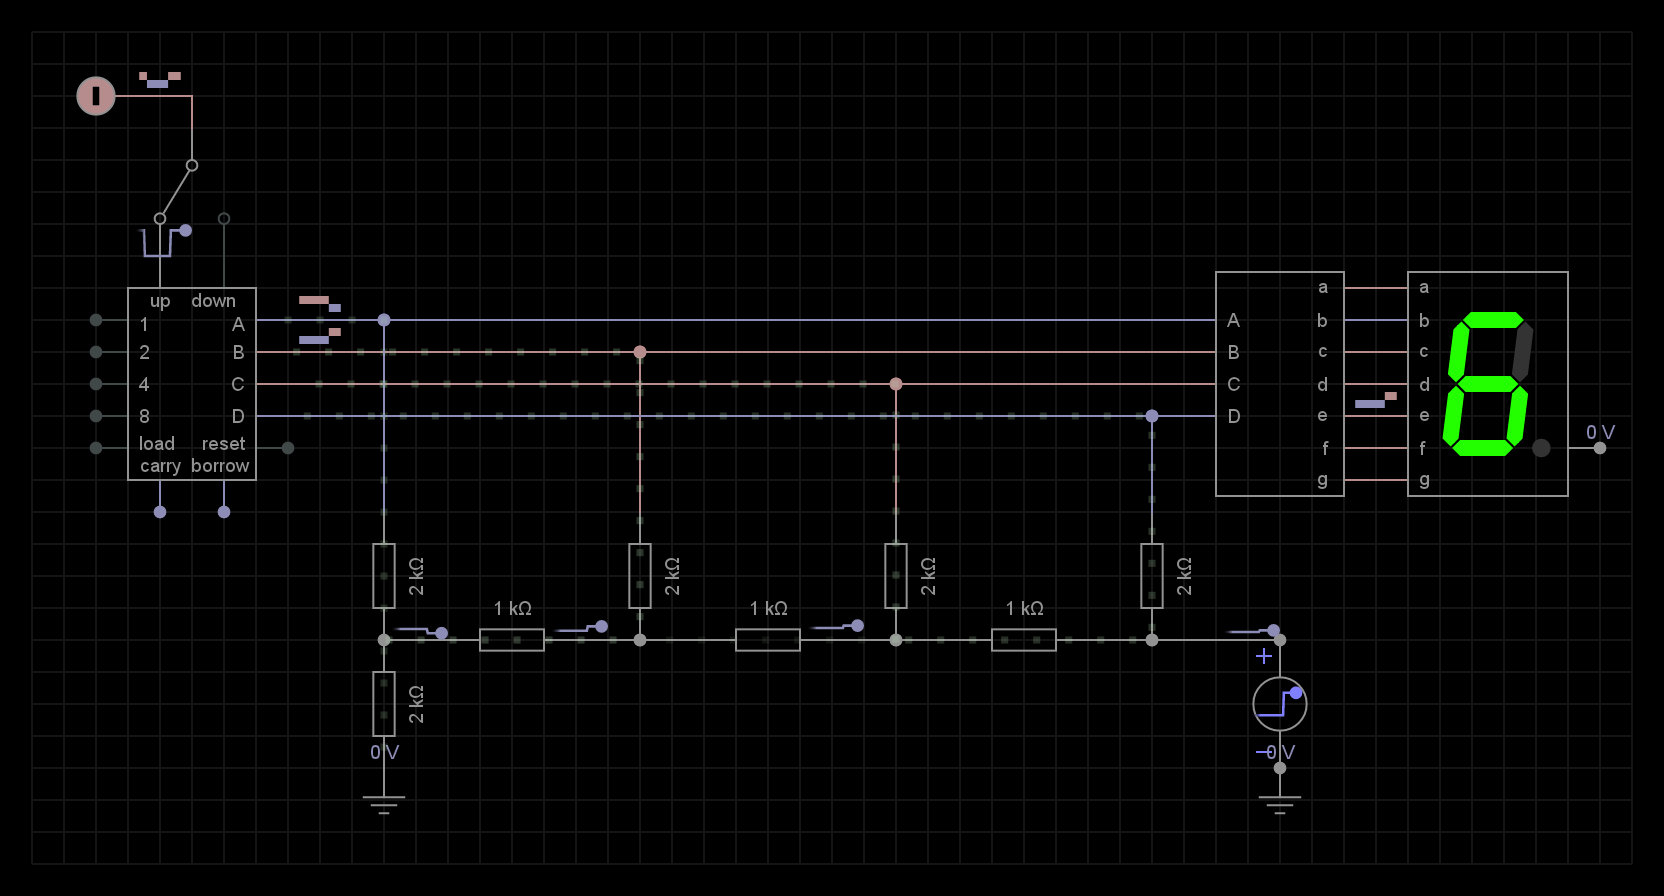
\includegraphics[width=1.05\textwidth]{circuit(4).png}
 \caption{Примерная схема имплантированного R2R преобразователя, преобразователь на чипе способен выдавать 64-256 напряжений от $ 0 $ до $ V_{dd}=2.5V $ }
 \end{figure}
 \end{center}
}











\frame{\frametitle{ИСТОЧНИКИ}
 \begin{itemize}
 	\item{\small Mitigating wakeup effect and improving
endurance of ferroelectric $Hf_{0.5}Zr_{0.5}O_2$ thin
films by careful La-doping Published Online: 15 January 2019}
	\item {\small Improved Ferroelectric Switching Endurance of La-Doped $Hf_{0.5}Zr_{0.5}O_2$
Thin Films
Anna G. Chernikova, Maxim G. Kozodaev, Dmitry V. Negrov, Evgeny V. Korostylev,
Min Hyuk Park, Uwe Schroeder, Andrey M. Markeev}
   \item {\small Advanced Circuit Design of Gigabit-Density FRAM
Von der Fakultät für Elektrotechnik und Informationstechnik der Rheinisch-Westfälischen Technischen Hochschule Aachen zur Erlangung des akademischen Grades eines Doktors Dissertation}
   \item { \small Physics of ferroelectrics PBLittlewood January 27, 2002 }
	\item The beamer class
User Guide for version 3.55.
   
 \end{itemize}
}













\end{document}